\documentclass[tikz, border=3pt]{standalone}

\usepackage{tikz}
\usepackage{pgfplots}

\begin{document}
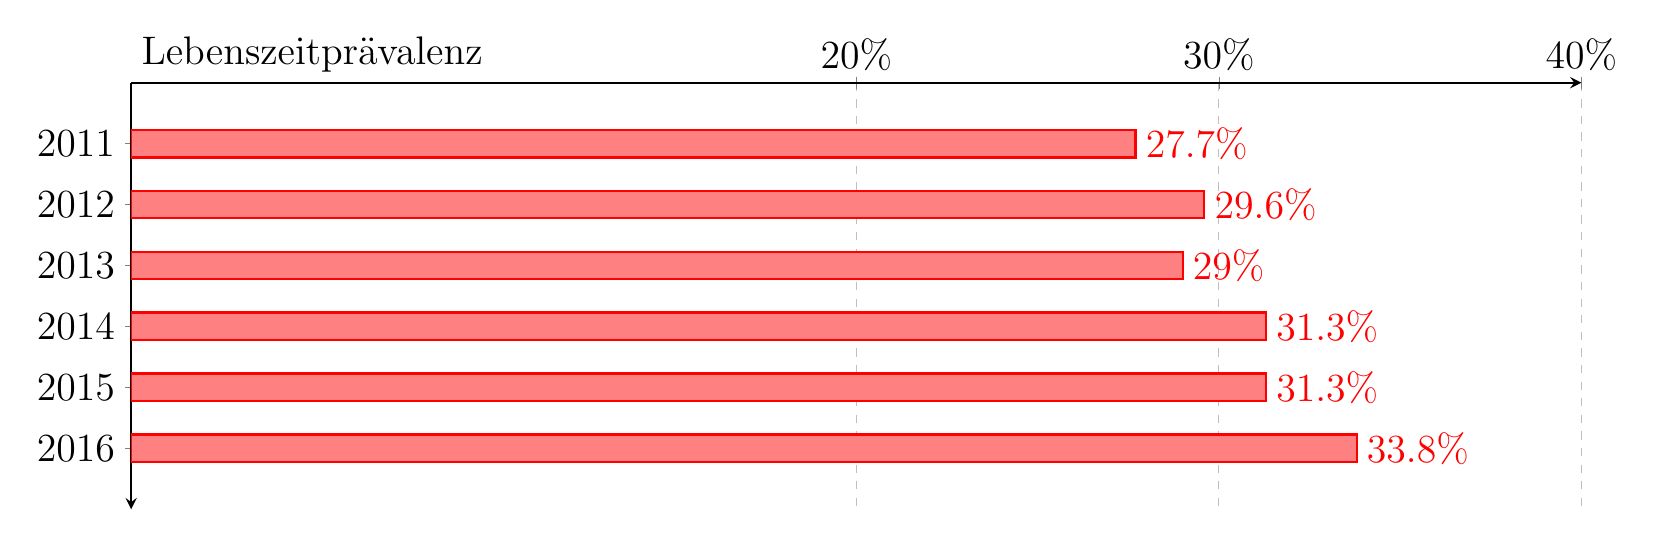
\begin{tikzpicture}

\begin{axis}[
	thick,
	xbar,
	xmin=0, xmax=40,
	ymin=0, ymax=7,
	width=20cm,
	height=7cm,
	xlabel = {\Large Lebenszeitprävalenz},	
	xtick={20,30,40},
    ytick = {1,2,3,4,5,6},
	yticklabels={
		\Large 2011,
		\Large 2012,
		\Large 2013,
		\Large 2014,
		\Large 2015,
		\Large 2016		
	},
	y dir=reverse,
	x tick label style={yshift=1mm,anchor=south},
	xticklabel={\Large\pgfmathprintnumber\tick\%},
	axis lines=middle,
    xmajorgrids,
    grid style={dashed},
    every axis x label/.style={
        at={(ticklabel* cs:0)},
        anchor=south west,
	},
]


	
% Cannabis
\addplot[ 
	color=red,
	fill=red!50!,
	bar width=10pt,
	nodes near coords=\Large\pgfmathprintnumber{\pgfplotspointmeta}\%,
] coordinates {
	(27.7, 1)
	(29.6, 2)
	(29.0, 3)
	(31.3, 4)
	(31.3, 5)
	(33.8, 6)
};


\end{axis}

\end{tikzpicture}
\end{document}